\documentclass{beamer}
\setbeamertemplate{section in toc}[sections numbered]
\usefonttheme[onlymath]{serif}
\beamertemplatenavigationsymbolsempty
\setbeamertemplate{footline}{% 
  \hfill% 
  \usebeamercolor[gray!50]{page number in head/foot}% 
  \usebeamerfont{page number in head/foot}% 
  \insertframenumber\,/\,\inserttotalframenumber%
}
\usepackage{amsmath}
\usepackage{graphicx}
\usepackage{lmodern}
\usepackage[round]{natbib}
\usepackage{tabularx}
\usepackage{physics}
\usepackage{color}
\usepackage{bm}
\usepackage{amssymb}
\usepackage{bbold}
\usepackage{tikz}
\usepackage{empheq}
\usepackage{stackengine}
\usepackage{framed}
\usepackage[percent]{overpic}
\usepackage[export]{adjustbox}
\usepackage{simpler-wick}
\DeclareMathOperator{\sgn}{sgn}
\tikzset{>=latex}
\newcommand{\blue}[1]{{\color{blue}{#1}}}
\newcommand{\md}{\mathrm{d}}
\newcommand{\ms}{\mathsf}
\newcommand{\bs}{\boldsymbol}
\newcommand{\mc}{\mathcal}
\renewcommand{\(}{\left(}
\renewcommand{\)}{\right)}
\renewcommand{\[}{\left[}
\renewcommand{\]}{\right]}

%Information to be included in the title page:
\title{Higher-order topology in condensed matter systems}
%\author{Apoorv Tiwar, Ammar Jahin, and Yuxuan Wang}
%\institute{University of Florida}
\date{University of Florida, November}

\begin{document}
\frame{\titlepage} 

\begin{frame}
    \frametitle{Outline}

    \tableofcontents
\end{frame}

\section{Introduction---Band topology}
\begin{frame}
    \frametitle{Bands structure}
    Electrons on a lattice can be described by local degrees of freedom, 
    \begin{columns}
        \begin{column}{0.7\textwidth}
            \begin{align*}
                \ket{\bm R \ i} 
            \end{align*}
            \vfill
        \end{column}
        \begin{column}{0.3\textwidth}
            \centering
            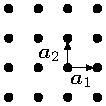
\includegraphics[]{square_lattice.pdf}
            \vfill
        \end{column}
    \end{columns}
    \begin{itemize}
        \item $\bm R$ donate lattice coordinate.
        \item $i$ donate (pseudo)spin degrees of freedom.
    \end{itemize} \pause
    For free electrons, 
    \begin{columns}
        \begin{column}{0.7\textwidth}
            \begin{align*}
                \ket{\bm k\  i} = \sum_{\bm R} e^{i\bm k \cdot \bm R} \ket{\bm R \ i} \\
                \mel*{\bm k^\prime \ i}{H}{\bm k \ j} = \mc H^{ij}(\bm k) \delta_{\bm k, \bm k^\prime}
            \end{align*}
            \vfill
        \end{column}
        \begin{column}{0.3\textwidth}
            \centering
            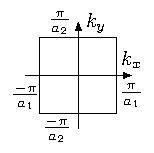
\includegraphics[]{square_recep_lattice.pdf}
            \vfill
        \end{column}
    \end{columns}
    \begin{itemize}
        \item Translational symmetry $\rightarrow$ conservation of crystal momentum.
        \item Diagonalizing the Hamiltonian we end up with a set of bands. 
        \item We will refer to $\mc H(\bm k)$ as the Hamiltonian.
        \item We are interested in gapped systems (insulators).
    \end{itemize}
\end{frame}
\begin{frame}
    \frametitle{Topology of the occupied bands}
    Suppose we are studying systems with some symmetry group. Define an equivalence between $\mc H^0(\bm k)$ and $\mc H^1(\bm k)$:
    \begin{framed}
        \begin{center}
            $\mc H^0(\bm k) \approx \mc H^1(\bm k)$ iff $\exists$
        \end{center}
        \begin{itemize}
            \item $\ \mc H(\bm k, t)$;  $\mc H(\bm k,0) = \mc H^0(\bm k)$, $\mc H(\bm k,1) = \mc H^1(\bm k)$, 
            \item $\mc H(\bm k,t)$ for all values of $t \in [0,1]$ is: 
            \begin{enumerate}
                \item Gapped
                \item Preserve the symmetry
            \end{enumerate}
        \end{itemize}
    \end{framed}  \pause
    \begin{itemize}
        \item This can be thought as deforming the occupied (and empty bands) bands from those of $\mc H^0(\bm k)$ to those of $\mc H^1(\bm k)$. 
        \item If this deformation is possible, then the occupied bands of $\mc H^0(\bm k)$ and $\mc H^1(\bm k)$ are topologically equivalent.
    \end{itemize}
\end{frame}

\begin{frame}
    \frametitle{Topological classification}

    \begin{itemize}
        \item Topological classification require a survey of all possible gapped Hamiltonian and grouping them into equivalence classes under the restrictions of some symmetry group. 
    \end{itemize}
    \centering
    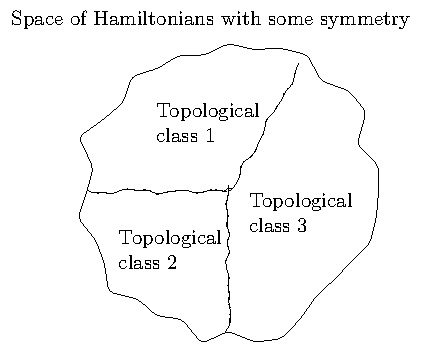
\includegraphics[]{hams_space.pdf}
    \begin{itemize}
        \item Find topological invariants that differentiate one class from the other. 
    \end{itemize}


\end{frame}


\begin{frame}
    \frametitle{Internal symmetries}
    \begin{framed}
        Internal symmetries are those that do not change the positions of the particles: $\bm R \rightarrow \bm R$. 
    \end{framed}
    \pause
    \begin{columns}
        \begin{column}{0.5\textwidth}
            Three important internal symmetries: 
            \begin{itemize}
                \item Time-reversal symmetry ($\mc T$)
                \item Particle-hole symmetry ($ \mc P$)
                \item Chiral symmetry ($\mc C$)
            \end{itemize}
            \begin{framed}
                Complete topological classification exists for the $10$ AZ classes.
            \end{framed}
        \end{column}\pause
        \begin{column}{0.5\textwidth}
            \begin{table}[t]
                \centering
                \begin{tabularx}{0.95\textwidth}{>{\centering\arraybackslash}X |>{\centering\arraybackslash}X |>{\centering\arraybackslash}X |>{\centering\arraybackslash}X}
                    \hline
                    \hline
                    \rule{0pt}{3ex}   
                    AZ  & $\mc T^2$ & $\mc P^2$ & $\mc C^2$ \\
                    \hline  
                    A   &    0      &0          & 0  \\       
                    AIII&    0      &0          & 1  \\         
                    \hline 
                    AI  &    1      &  0        & 0  \\         
                    BDI &    1      &  1        & 1  \\         
                    D   &    0      &  1        & 0  \\         
                    DIII&   -1      &  1        & 1  \\         
                    AII &   -1      &  0        & 0  \\         
                    CII &   -1      & -1        & 1  \\         
                    C   &    0      & -1        & 0  \\         
                    CI  &    1      & -1        & 1  \\         
                \end{tabularx} 
            \end{table}
        \end{column}
    \end{columns}
\end{frame}

\begin{frame}
    \frametitle{Gapless boundaries}
    \begin{center}
        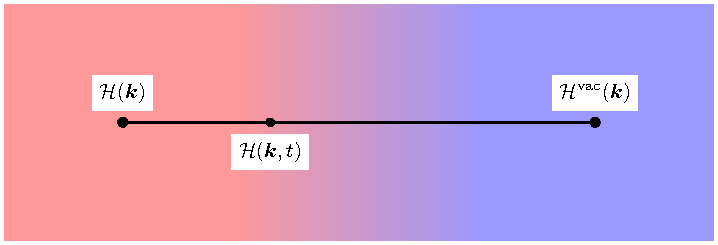
\includegraphics[scale = 0.88]{smooth_boundary.pdf}
    \end{center}
    \begin{itemize}
        \item A boundary interpolates between a topological system and the vacuum. 
        \item Internal symmetries are not broken on the boundary.
    \end{itemize}
    \pause
    \begin{framed}
        Topological systems protected by internal symmetries \emph{only} will in general have gapless boundaries. 
    \end{framed}
\end{frame}

\begin{frame}
    \frametitle{Examples}
    \begin{columns}
        \begin{column}{0.6\textwidth}
            \underline{In $2$D:}\\
            Chern insulators. \\
            Protecting symmetries: None. \\
            Topological invariant: Chern number.
        \end{column}
        \begin{column}{0.4\textwidth}
            \begin{center}
                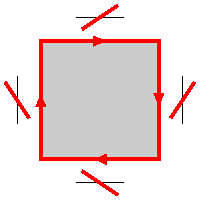
\includegraphics[valign=c]{first_order_boundary.pdf} 
            \end{center}
        \end{column}
    \end{columns}
    \pause
    \begin{columns}
        \begin{column}{0.6\textwidth}
            \underline{In $1$D:}\\
            SSH chain. \\
            Protecting symmetry: Chiral symmetry\\
            Topological invariant: Polarization 
        \end{column}

        \begin{column}{0.4\textwidth}
            \begin{center}
                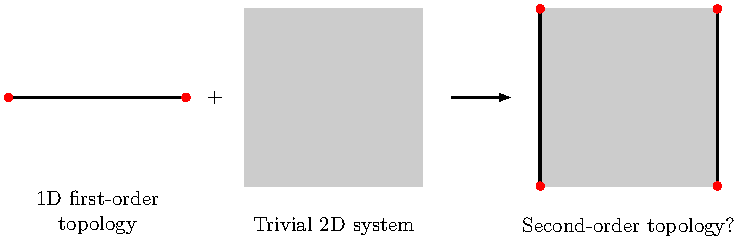
\includegraphics[scale=0.88, trim = 0 50 265 10, clip, valign=c]{cheap_corner.pdf}
            \end{center}
        \end{column}
    \end{columns}


\end{frame}


% \begin{frame}
%     \frametitle{Examples}

%         \begin{table}[t]
%         \centering
%         \begin{tabularx}{\textwidth}{>{\centering\arraybackslash}X@{} >{\centering\arraybackslash}X@{}  >{\centering\arraybackslash}X@{}  >{\centering\arraybackslash}X | >{\centering\arraybackslash}X@{} >{\centering\arraybackslash}X@{}  >{\centering\arraybackslash}X@{}  >{\centering\arraybackslash}X@{} >{\centering\arraybackslash}X@{} >{\centering\arraybackslash}X@{}  >{\centering\arraybackslash}X@{}  >{\centering\arraybackslash}X}
%             \hline
%             \hline
%             \multicolumn{4}{>{\centering\setlength\hsize{0.33\textwidth} }X|}{Symmetry} & \multicolumn{8}{>{\centering\setlength\hsize{0.66\textwidth}}X}{$d$}\\
%             \rule{0pt}{3ex}   
%             AZ  & $\mc T^2$ & $\mc P^2$ & $\mc C^2$ & $0$ & $1$ & $2$ & $3$  & $4$ & $5$ & $6$ & $7$ \\
%             \hline  
%             A   &    0      &0          & 0 & $\mathbb{Z}$ &    0      &    $\mathbb{Z}$      & 0 & $\mathbb{Z}$   &    0  &$\mathbb{Z}$   & 0  \\       
%             AIII&    0      &0          & 1 & 0            &    $\mathbb{Z}$    &  0  & $\mathbb{Z}$ &  0  & $\mathbb{Z}$   &  0  & $\mathbb{Z}$  \\         
%             \hline 
%             AI  &    1      &  0        & 0 & $\mathbb{Z}$   &    0      &0          & 0  & $2\mathbb{Z}$   &    0    &$\mathbb{Z}_2$          & $\mathbb{Z}_2$  \\         
%             BDI &    1      &  1        & 1 & $\mathbb{Z}_2$   &    $\mathbb{Z}$      &0          & 0 & 0   &    $2\mathbb{Z}$      &0  & $\mathbb{Z}_2$  \\         
%             D   &    0      &  1        & 0 & $\mathbb{Z}_2$   &    $\mathbb{Z}_2$ & $\mathbb{Z}$   & 0 & 0   &    0      & $2\mathbb{Z}$  & 0  \\         
%             DIII&   -1      &  1        & 1 & 0   &    $\mathbb{Z}_2$   &$\mathbb{Z}_2$  & $\mathbb{Z}$ & 0   &    0      &0          & $2\mathbb{Z}$  \\         
%             AII &   -1      &  0        & 0 & $2\mathbb{Z}$   &  0   &$\mathbb{Z}_2$  & $\mathbb{Z}_2$ & $\mathbb{Z}$   &    0      &0          & 0  \\         
%             CII &   -1      & -1        & 1 & 0   &    $2\mathbb{Z}$  &  0 &$\mathbb{Z}_2$  & $\mathbb{Z}_2$ & $\mathbb{Z}$  &   0   &0          \\         
%             C   &    0      & -1        & 0 & 0   &    0      &$2\mathbb{Z}$  & 0 & $\mathbb{Z}_2$   &   $\mathbb{Z}_2$   &$\mathbb{Z}$  & 0  \\         
%             CI  &    1      & -1        & 1 & 0   &    0      &0   & $2\mathbb{Z}$ & 0   &  $\mathbb{Z}_2$  &   $\mathbb{Z}_2$   & $\mathbb{Z}$ \\         
%         \end{tabularx} 
%     \end{table}


% \end{frame}

\AtBeginSection[]
{\begin{frame}
    \frametitle{Outline}
    \tableofcontents[currentsection]
\end{frame}
}
\section{Higher-order topology and boundary obstructed topology}

\begin{frame}
    \frametitle{Higher-order topology}

    Can we find topological systems systems with gapped boundaries?
    \begin{columns}
        \begin{column}{0.5\textwidth}
            \begin{center}
                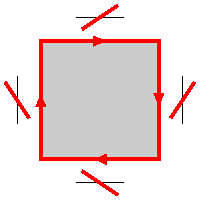
\includegraphics[valign=c]{first_order_boundary.pdf} 
            \end{center}
            First-order topology; gapless mode on boundaries of co-dimension 1. 
        \end{column}
        \begin{column}{0.5\textwidth}
            \begin{center}
                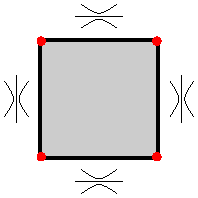
\includegraphics[valign=c]{second_order_surface.pdf}
            \end{center}
            Second-order topology; gapless mode on boundaries of co-dimension 2. 
        \end{column}
    \end{columns} 
    \begin{framed}
        The protecting symmetry must be broken on the boundary. Internal symmetries are not enough. 
    \end{framed}
\end{frame}

\begin{frame}
    \frametitle{Spacial symmetries}

    \begin{framed}
        Spacial symmetries are those that change the position of the particles. $\bm R \rightarrow \bm R^\prime$.
    \end{framed}
    Examples of spacial symmetries: 
    \begin{align*}
        C_4 : (R_x, R_y) \rightarrow (-R_y, R_x) && C_2 : (R_x, R_y) \rightarrow (-R_x, -R_y)
    \end{align*}
    \centering
    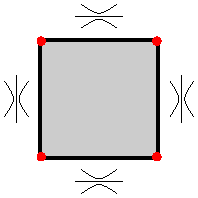
\includegraphics[]{second_order_surface.pdf}

    $C_4$ and $C_2$ are broken on the boundaries.  
\end{frame}

\begin{frame}
    \frametitle{A cheap way to get corner modes}
    \begin{center}
        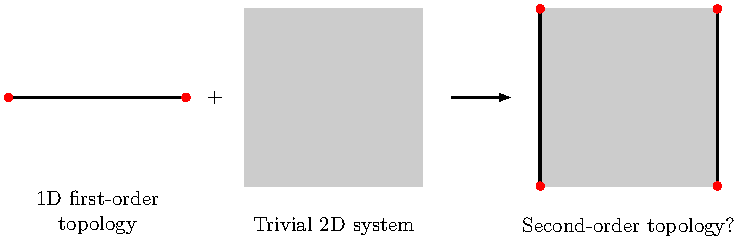
\includegraphics[scale=0.85]{cheap_corner.pdf}
    \end{center}
    \begin{itemize}
        \item These corner zero modes are not protected by a bulk gap closing. 
    \end{itemize}

\end{frame}

\begin{frame}
    \frametitle{Higher-order and boundary-obstructed topologies}
    \centering 
    
\includegraphics[]{seond_order_boudary.pdf}

    \vspace{5pt}
    Second-order topology 
    \vfill
    
\includegraphics[]{boundary_obstructed.pdf}

    \vspace{5pt}
    Boundary-obstructed topology

    \begin{itemize}
        \item What kinds of system would show such surface signature?
        \item What kinds of topological invariants we can find?
    \end{itemize}

\end{frame}



\section{Chiral Dirac superconductors}


\begin{frame}
    \frametitle{Superconductors}
    The BdG form for superconducting Hamiltonian, 
    \begin{align*}
        H =\frac{1}{2}\int \frac{d\bm k}{(2\pi)^{d}}  \  \mqty{\mqty[\Psi^\dagger(\bm k)  \Psi(-\bm k)] \\ \mbox{}}
        \mqty[\mc H_n(\bm k) && \Delta(\bm k) \\ 
        \Delta^\dagger (\bm k) && -\mc H^*_n(-\bm k)] \mqty[\Psi(\bm k) \\ 
        \Psi^\dagger(-\bm k)]
    \end{align*}
    \begin{itemize}
        \item $\Psi^\dagger(\bm k) = (a_1(\bm k), \dots, a_N(\bm k))$.
        \item $\mc H_n(\bm k)$ is the normal state Hamiltonian.
        \item $\Delta(\bm k)$ is the superconducting order parameter.
        \item The BdG Hamiltonian $ \mc H(\bm k) = \mqty[\mc H_n(\bm k) && \Delta(\bm k) \\ 
        \Delta^\dagger (\bm k) && -\mc H^*_n(-\bm k)]$ allows us to study the topology of superconductors within the same framework as insulating Hamiltonians. 
        \item BdG Hamiltonians has an \emph{intrinsic} particle-hole symmetry. 
    \end{itemize}
\end{frame}

\begin{frame}
    \centering
    \begin{columns}
        \begin{column}{0.5\textwidth}
            \centering
            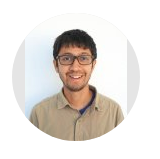
\includegraphics[trim= 0 20 0 20,clip]{Screenshot_20200516_213116.png}

            Apoorv Tiwari
            
            University of Zurich
        \end{column}
        \begin{column}{0.5\textwidth}
            \centering
            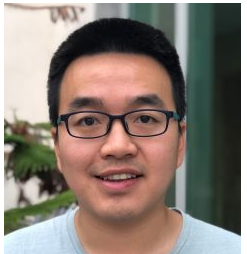
\includegraphics[scale=0.4]{YWSC.png}

            Yuxuan Wang 

            University of Florida
        \end{column}
    \end{columns}
\end{frame}

\begin{frame}
    \frametitle{Chiral Dirac superconductors}

    Can we find a low energy criteria that guarantee the existence of the corner modes? 
    \vspace{10pt}
    \begin{columns}
        \begin{column}{0.5\textwidth}
            \underline{In $2$D}
            \begin{itemize}
                \item Dirac points in the normal state.
                \item A $p+ip$ superconducting order parameter gapping the Dirac points.
                \item With $C_4$ symmetry $\rightarrow$ second-order topology 
                \item With $C_2$ symmetry $\rightarrow$ boundary-obstructed topology. 
            \end{itemize}
        \end{column}
        \begin{column}{0.5\textwidth}
            \centering 
            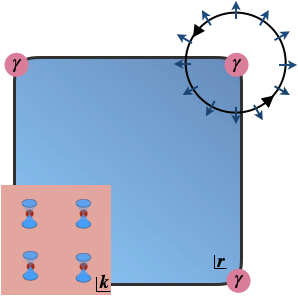
\includegraphics[scale = 0.5]{HOTSc3.png}
        \end{column}
    \end{columns}

\end{frame}


\begin{frame}
    \frametitle{Summary}

    \begin{itemize}
        \item Topological band systems are those that cannot be deformed to the vacuum without: \begin{enumerate}
            \item Closing a gap
            \item Breaking the symmetry
        \end{enumerate}
        \item Topologies protected by internal symmetries alone lead to first-order topology (gapless boundaries). 
        \item Including spacial symmetries can lead to a much richer topological structure. 
        \item Higher-order topologies have gapless modes on boundaries with co-dimension higher than one. 
        \item Boundary-obstructed topologies are only protected by a boundary gap closing. 
    \end{itemize}    

\end{frame}


% \begin{frame}
%     \frametitle{Everyday tools}

%     \begin{itemize}
%         \item Quantum mechanics \\ 
%         Not much field theory 
%         \item Python (or Matlab, or Mathematica) \\ 
%         Making tight binding models and solve for zero modes. 
%     \end{itemize}

% \end{frame}

% \begin{frame}
%     \frametitle{A concrete model}

%     \begin{align*}
%         \mc H(\bm k) = &\[\gamma_x + \cos(k_x)\] \sigma_x \tau_z + \[\gamma_y + \cos(k_y)\] \sigma_z \tau_z -\mu \tau_z  \nonumber \\
%         & + \Delta \sin(k_x) \tau_y + \Delta \sin(k_y) \tau_x 
%     \end{align*}
%     \begin{align*}
%         &C_4 \mc H(k_x, k_y) C_4^{-1} = \mc H(-k_y, k_x) && C_4 = \frac{1}{\sqrt{2}} (\sigma_x + \sigma_y) e^{-i\frac{\pi}{4}\tau_z} \nonumber \\ 
%         &\mc P \mc H(\bm k) \mc P^{-1} = -\mc H(-\bm k) && \mc P = \tau_x K 
%     \end{align*}
%     \centering
%     $4$ Majorana corner zero modes. 

%     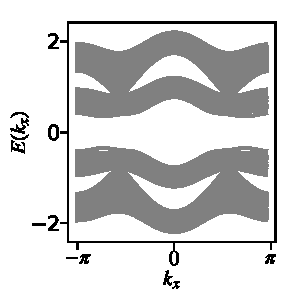
\includegraphics[scale=0.7, trim = 5 0 10 0,clip, valign=c]{super_4_energy_cylinder.pdf}
%     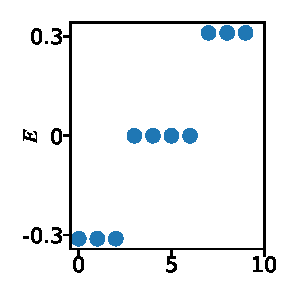
\includegraphics[scale=0.7, trim = 9 0 10 0,clip, valign=c]{super_4_open_boundary_zero_modes.pdf}
%     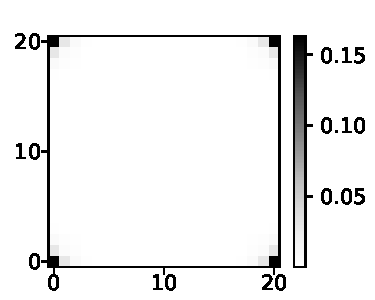
\includegraphics[scale=0.62, trim = 0 0 0 15, clip, valign=c]{super_4_open_boundary_zero_modes_real_space.pdf}

%     $\gamma_x = \gamma_y = 0.2,\  \Delta = 0.4,\  \mu = 0.5 $
% \end{frame}

% \begin{frame}
%     \frametitle{A more general model---a sufficient condition }
%     \begin{columns}[t]
%         \begin{column}{0.6\textwidth}
%             $\mc H(\bm k) = f_1(\bm k) \sigma_x \tau_z + f_2(\bm k) \sigma_z \tau_z -\mu \tau_z $
%             \centering
%             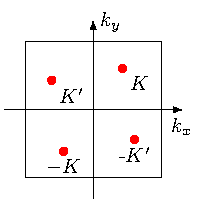
\includegraphics[]{normal_stateBZ.pdf}
%         \end{column}
%         \begin{column}{0.4\textwidth}
%             $+ \Delta_1(\bm k) \tau_y + \Delta_2(\bm k) \tau_x$

%             \vspace{20pt}
%             $p+ip$ order parameter. 
%         \end{column}
%     \end{columns}
%     \begin{framed}
%         \begin{itemize}
%             \item With $C_4$ symmetry the model has a second-order topological phase with corner Majorana zero modes. 
%             \item With only $C_2$ symmetry the model has a boundary-obstructed phase with corner Majorana zero modes.
%         \end{itemize}
%     \end{framed}
% \end{frame}


% \begin{frame}
%     \frametitle{Symmetry indicator method}
%     \begin{align*}
%         \mc H(\bm k) = f_1(\bm k) \sigma_x \tau_z + f_2(\bm k) \sigma_z \tau_z -\mu \tau_z + \Delta_1(\bm k) \tau_y + \Delta_2(\bm k) \tau_x
%     \end{align*}
%     \begin{columns}[c]
%         \begin{column}{0.5\textwidth}
%             Points in the BZ invariant under $C_4$: $\bm k^* = \{(0,0), (\pi,\pi)\}$
%             \begin{align*}
%                 &\[C_4, H(\bm k^*)\] = 0 \\ 
%                 &f_1(0,0) = f_2(0,0) = f_\Gamma \\
%                 &f_1(\pi,\pi) = f_2(\pi,\pi) = f_M \\
%             \end{align*}

%             Points in the BZ only invariant under $C_2$: $\bm k^* = \{(\pi,0), (0,\pi)\}$
%             \begin{align*}
%                 \[C_2, H(\bm k^*)\] = 0 \\
%             \end{align*}
%         \end{column}
%         \begin{column}{0.5\textwidth}
%             \centering
%             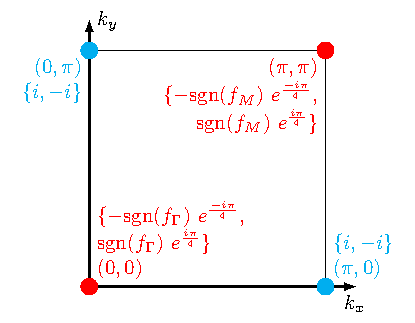
\includegraphics[scale = 0.75]{super_4_wannier_rep.pdf}
%             Symmetry operators eigenvalues at the high-symmetry points are topological invariants.
%         \end{column}
%     \end{columns}
% \end{frame}

% \begin{frame}
%     \frametitle{Wannier centers}
%     Disclaimer: We first ignore the fact that we are dealing with a BdG Hamiltonian and treat it like a regular insulator.  We study the system at half-filling with $2$ \emph{electrons} per unit cell.
%     \begin{columns}[c]
%         \begin{column}{0.75\textwidth}
%             \begin{framed}
%                 If a well localized Wannier representation exists, the Wannier centers must (1) respect the symmetry of the system, and (2) reproduce the same symmetry operators.
%             \end{framed}
%         \end{column}
%         \begin{column}{0.25\textwidth}
%             \centering
%             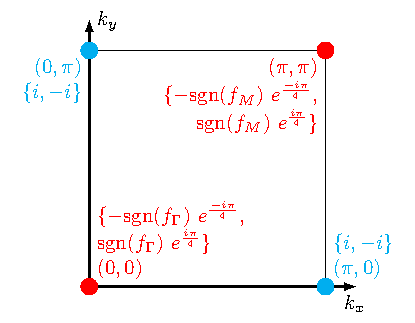
\includegraphics[scale = 0.385]{super_4_wannier_rep.pdf}
%         \end{column}
%     \end{columns}
%     \begin{columns}[c]
%         \begin{column}{0.35\textwidth}
%             \centering 
%             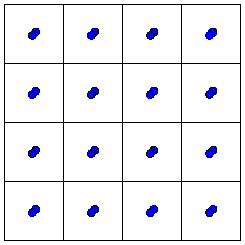
\includegraphics[scale=0.65]{atomic_limit_zero.pdf}
%             $\sgn(f_\Gamma)\sgn(f_M) = 1$
%         \end{column}
%         \begin{column}{0.65\textwidth}
%             \centering
%             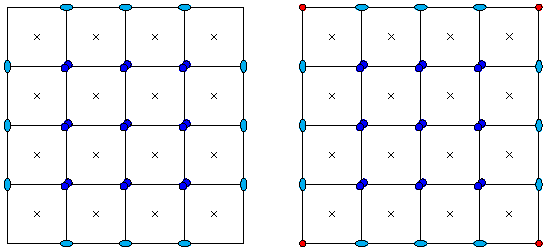
\includegraphics[scale=0.65]{atomic_limit_half.pdf}
%             $\sgn(f_\Gamma)\sgn(f_M) = -1$
%         \end{column}
%     \end{columns}

% \end{frame}

% \begin{frame}
%     \frametitle{Filling anomaly---Majorana corner modes}
%     \begin{columns}[b]
%         \begin{column}[c]{0.4\textwidth}
%             \begin{framed}
%                 Filling anomaly means the system cannot be: 
%                 \begin{enumerate}
%                     \item Neutral
%                     \item Gapped 
%                     \item $C_4$ symmetric
%                 \end{enumerate}
%             \end{framed}
                            
%             \hspace{20pt}
%         \end{column}
%         \begin{column}[c]{0.6\textwidth}
%             \centering
%             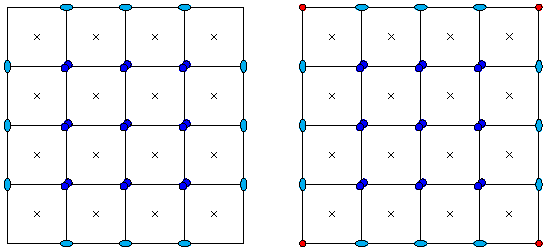
\includegraphics[scale=0.65]{atomic_limit_half.pdf}
%             One orbital at each corner that can be either empty, or filled.
%         \end{column}
%     \end{columns}

%     What does the filling anomaly mean for the BdG Hamiltonian? 
%     \begin{itemize}
%         \item Filling anomaly means one state localized at each corner.  
%         \item Particle-hole symmetry is a local symmetry.
%         \item If $\ket{\Psi}$ is localized on one corner, so is $\ket{\mc P \Psi}$.
%         \item It must be that $\ket{\mc P\Psi} \propto \ket{\Psi}$; A Majorana zero mode. 
%     \end{itemize}
% \end{frame}

% \begin{frame}
%     \frametitle{Is the system in the topological phase?}
%     The condition for the topological phase is $\sgn(f_\Gamma)\sgn(f_M) = -1$. Is it true for our system? 
%     \begin{columns}[]
%         \begin{column}{0.5\textwidth}
%             \vspace{5pt}

%             $\mc H_n(\bm k) = f_1(\bm k) \sigma_x + f_2(\bm k) \sigma_z$
%             \hspace{1pt} 
%             \begin{itemize}
%                 \item The Dirac point is a source of \emph{magnetic} field.
%                 \item Berry phase gained when moving around the loop is $\pi$.
%             \end{itemize}
%             \begin{align*}
%                 \hat{\bm n}(\bm k) \equiv \frac{f_1(\bm k) e_x + f_2(\bm k) e_z}{\sqrt{f_1^2(\bm k) + f_2(\bm k)}}
%             \end{align*}
%         \end{column}
%         \begin{column}{0.5\textwidth}
%             \centering
%             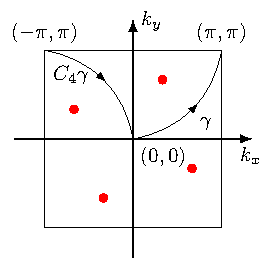
\includegraphics[]{BZ_path.pdf}
%         \end{column}
%     \end{columns}
%     \begin{framed}
%         \centering
%         $N_\text{w} (\gamma \circ C_4 \gamma) = 2N_{\text{w}}(\gamma) = 2\pi$

%         $\hat{\bm n}(0,0) = -\hat{\bm n}(\pi, \pi)$
%     \end{framed}
% \end{frame}

% \begin{frame}
%     \frametitle{Boundary-obsruction---surface defect approach}
%     \begin{framed}
%         When $C_4$ is broken down to $C_2$ we no longer have a phase protected by bulk gap closing.
%     \end{framed}
%     Our approach: 
%     \begin{enumerate}
%         \item Solve for the boundary theory knowing the low energy properties of the model.
%         \item Show that the boundary properties, as derived from the bulk, lead to a Majorana corner zero mode. 
%     \end{enumerate}
%     \begin{columns}[]
%         \begin{column}{0.4\textwidth}
%             \begin{itemize}
%                 \item Solve for the surface theory at each \emph{point} on the rounded corner.
%             \end{itemize}
%         \end{column}
%         \begin{column}{0.6\textwidth}
%             \centering 
%             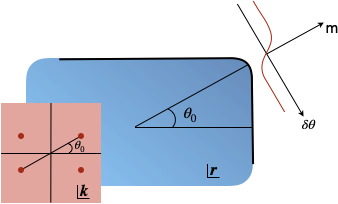
\includegraphics[scale = 0.5]{corner_without_C4.png}
%         \end{column}
%     \end{columns}
% \end{frame}


% \begin{frame}
%     \frametitle{Surface theory}
%     \begin{center}
%         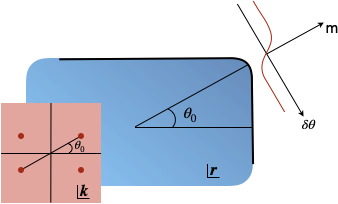
\includegraphics[scale = 0.3]{corner_without_C4.png} \hspace{10pt}
%         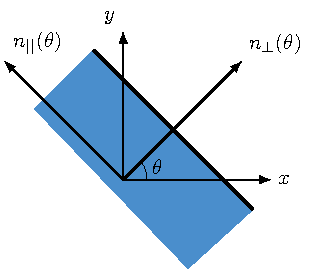
\includegraphics[scale = 0.5]{boundary_directions.pdf}
%     \end{center}

%     \begin{itemize}
%         \item $k_{\perp}(\theta)$ is not conserved, $k_{||}(\theta)$ is. 
%         \item For small paring terms, the low energy theory of the system is near the Dirac points.
%         \item For $\theta = \theta_0$, and $k_{||}(\theta_0) = 0$, the system has $2$ zero modes:
%     \end{itemize}
%     \begin{align*}
%         \psi^\alpha(\bm r) = \chi^\alpha \sin(|\bm K| \ r_{\perp})\  e^{\Delta_0  r_\perp / v_{\perp}}, \ \ \  \alpha \in \{0,1\}
%     \end{align*}
%     \centering

% \end{frame}

% \begin{frame}
%     \frametitle{Surface theory}
%     Make two different perturbations:
%     \begin{columns}[]
%         \begin{column}{0.5\textwidth}
%             \centering
%             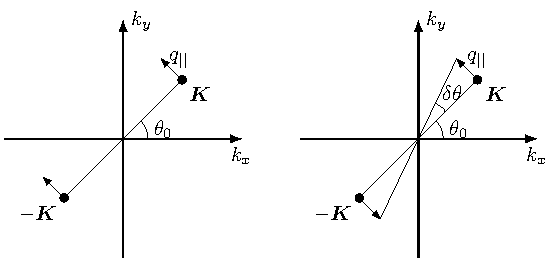
\includegraphics[scale=0.73, trim= 0 0 150 0,clip]{small_q_diviations.pdf}

%             A small momentum deviation to get the dispersion. 
%         \end{column}
%         \begin{column}{0.5\textwidth}
%             \centering 
%             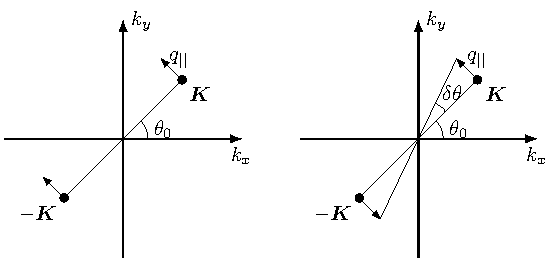
\includegraphics[scale=0.73, trim= 150 0 0 0,clip]{small_q_diviations.pdf}

%             A small $\delta \theta$ deviation to get the the surface theories at angles $\theta = \theta_0 +\delta \theta$
%         \end{column}
%     \end{columns}
%     \begin{framed}
%         \centering
%         $h(q_{||}, \delta \theta) = \alpha q_{||} s_1 + \beta \delta \theta s_2 $
%     \end{framed}
    
%     \begin{itemize}
%         \item Looks like a $1D$ Dirac equation with a mass domain wall, which we know host a zero mode at the domain wall. 
%     \end{itemize}
% \end{frame}

% \begin{frame}
%     \frametitle{Conclusions}

%     \begin{itemize}
%         \item In $2$D, we establish the 'Dirac + $p+ip$' as sufficient condition for higher-order and boundary obstructed topology. 
%         \item With a $C_4$ symmetry, the system is in a second-order topological phase. 
%         \item With only $C_2$ symmetry rhe system is in a boundary-obstructed phase. 
%     \end{itemize}
% \end{frame}

% \begin{frame}
%     \frametitle{Future work}

    

% \end{frame}
\end{document} 